\cotefile{73}
\scanpage{18}
\mspage{4}

% top centre
\unsure{quadrilatère}

% upper left
\figure{\begin{tikzpicture}[x=.83cm,y=.83cm,>=stealth]
\draw[->] (-2.6,-.06)--(3.25,.14);
\draw[->] (-.87,-2.02)--(.78,2.32);
\fill (-1.38,-.01) circle (1.6pt) node[below=2pt] {$s_0$};
\draw (.01,.01) ++(1.72,.045) circle (1.6pt) node[below=2pt] {$s_2$};
\fill (-.46,-.93) circle (1.45pt) node[right] {$s_1$};
\fill (.47,1.52) circle (1.45pt) node[right] {$s_3$};
\end{tikzpicture}}

% upper half, coordinate rows 1–4
\[
\begin{aligned}
(\unsure{a|\alpha}-1,\deleted{\unsure{a+1|a+}}0)&\qquad (-(a-1),b-1)=(-a+1,b-1) &&u_0\\
(0,b-1)&\qquad (a+1,-(b-1))=(a+1,-b+1) &&u_1\\
(a+1,0)&\qquad (-(a+1),b+1)=(-a-1,b+1) &&u_2\\
(0,b+1)&\qquad (a-1,-(b+1))=(a-1,-b-1) &&u_3
\end{aligned}
\]

% middle, product rows 1–4
\[
\begin{aligned}
(1-a)(1-b)+(1-b)(a+1)&=2(1-b)=f_{\unsure{1}}\\
(a+1)(b+1)+(a+1)(\deleted{\unsure{b}}1-b)&=2(a+1)=f_2\\
(a+1)(b+1)+(b+1)(1-a)&=2(b+1)=f_3\\
(a-1)(b-1)\deleted{\unsure{+}}\unsure{-}(b+1)(a-1)&=2(1-a)=f_0
\end{aligned}
\]

% below products, two columns
\[
f_1+f_3=f_2+f_0=\deleted{4}\unsure{v|\nu}
\quad\Big/\quad
\begin{aligned}
 f_3-f_1&=\text{\textcircled{$b$}}v\\
 f_2-f_0&=\text{\textcircled{$a$}}v
\end{aligned}
\]

% lower left, beside wedge identity
\figure{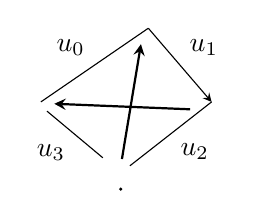
\begin{tikzpicture}[scale=.78,>=stealth]
\draw (-1.4,0)--(.35,1.2) node[midway,above left] {$u_0$};
\draw[->] (.35,1.2)--(1.38,0) node[midway,above right] {$u_1$};
\draw (1.38,0)--(.05,-1.04) node[midway,below right] {$u_2$};
\draw (-.39,-.91)--(-1.30,-.15) node[midway,below left] {$u_3$};
\draw[->,thick] (1.03,-.12)--(-1.18,-.03);
\draw[->,thick] (-.08,-.93)--(.23,.94);
\fill (-.1,-1.42) circle (.8pt);
\end{tikzpicture}}

% lower third, beside and below quadrilateral
\[
\begin{aligned}
u_0\wedge u_1+u_2\wedge u_3&=u_1\wedge u_2+u_3\wedge u_0
 \overset{?}{=}\underbrace{(u_0+u_1)(u_1+u_2)}_{\begin{gathered}u_0\wedge u_1+u_0\wedge u_2\\{}+u_1\wedge u_2\end{gathered}}\\
u_3&=-(u_0+u_1+u_2)
\end{aligned}
\]

% lower third, line with cross-outs and pairing strokes
\[
\underbrace{u_0\wedge u_1}\deleted{\unsure{+}}\unsure{-|+}%
\underbrace{\underbrace{u_2\,(u_0}+u_1}+\deleted{u_2})
 =\underbrace{u_1\wedge u_2}+\underbrace{\underbrace{u_0\wedge(\deleted{u_0}+u_1}+u_2})
\]

% foot, right above long rule
\[
u_2\wedge\underbrace{(u_3+u_0+u_1)}_{-u_2}=0\qquad\text{\unsure{Ok|Oh}}
\]

% foot, left to right
\figure{\begin{tikzpicture}[x=.77cm,y=.72cm,>=stealth]
\draw (0,.2) .. controls (1,-.12) and (4.6,1.25) .. (6.6,.14) .. controls (8.5,-.7) and (10.6,-.53) .. (12,-.38);
\draw[->] (1.2,-.58)--(2.58,.53) node[midway,above left] {$u$};
\draw[->] (2.58,.53)--(3.17,-.53) node[midway,right] {$v$};
\end{tikzpicture}}

% foot left, below rule
\[
\deleted{u\wedge v=-(-v)\wedge(-u)}
\]

% foot centre
\figure{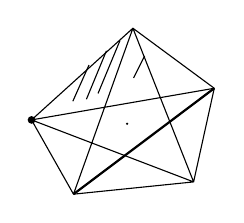
\begin{tikzpicture}[scale=.82]
\coordinate (a) at (-1.45,.08); \coordinate (b) at (.12,1.5);
\coordinate (c) at (1.38,.57); \coordinate (d) at (1.06,-.88); \coordinate (e) at (-.8,-1.07);
\draw (a)--(b)--(c)--(d)--(e)--cycle (a)--(c) (a)--(d) (b)--(d) (b)--(e) (e)--(c);
\draw[thick] (e)--(c); \fill (a) circle (1.7pt);
\draw (-.81,.37)--(-.56,.93) (-.60,.4)--(-.29,1.15) (-.42,.49)--(-.08,1.31) (.13,.73)--(.3,1.07);
\fill (.03,.02) circle (.55pt);
\end{tikzpicture}}

% archive sheet number: 24
\scanpage{19}
\mspage{5}

% top left
\figure{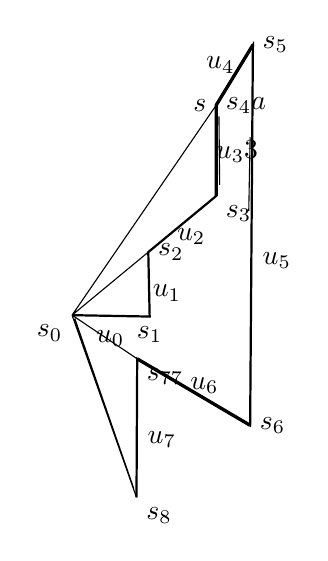
\begin{tikzpicture}[scale=.88]
\coordinate (a) at (0,0); \coordinate (b) at (1.12,-.02); \coordinate (c) at (1.1,.91);
\coordinate (d) at (2.08,1.72); \coordinate (e) at (2.08,3.03); \coordinate (f) at (2.61,3.9);
\coordinate (g) at (2.57,-1.59); \coordinate (h) at (.94,-.63); \coordinate (i) at (.93,-2.63);
\draw[thin] (a)--(c) (a)--(e) (a)--(h) (a)--(i) (.04,-.05)--(.89,-2.5);
\draw[thick] (a)--(b)--(c)--(d)--(e)--(f)--(g)--(h)--(i);
\draw[very thick] (d)--(e)--(f) (g)--(h); \draw (2.13,1.88)--(2.12,2.87) (2.55,1.5)--(2.57,2.57);
\node[below left] at (a) {$s_0$}; \node[below] at (b) {$s_1$}; \node[right] at (c) {$s_2$};
\node[below right] at (d) {$s_3$}; \node[right] at (e) {$s_{4}\unsure{a}$}; \node[left] at (e) {$s$};
\node[right] at (f) {$s_5$}; \node[right] at (g) {$s_6$}; \node[below right] at (h) {$s_{\deleted{\unsure{7}}7}$}; \node[below right] at (i) {$s_8$};
\node at (.55,-.34) {$u_0$}; \node at (1.37,.32) {$u_1$}; \node at (1.72,1.14) {$u_2$};
\node at (2.38,2.36) {$u_{3}\unsure{3}$}; \node at (2.14,3.61) {$u_4$}; \node[right] at (2.61,.79) {$u_5$};
\node at (1.91,-1.02) {$u_6$}; \node[right] at (.95,-1.8) {$u_7$};
\end{tikzpicture}}

% top right
\[
\boxed{\lambda_0=0}\Rightarrow u_1u_{0i}=\lambda_i u_{i-1}u_i
\]

% upper half, coordinate list
\[
\begin{aligned}
s_0&=(0,0)\\
s_1&=(1,0)\\
s_2&=(1,1) &&(y_2=1)\\
s_3&=(\beta_1,\beta_1) &&\beta_1\ne1,0\\
s_4&=(\beta_1,y_4) &&y_4\ne\beta_1\\
s_5&=(\beta_2\beta_1,\beta_2y_4) &&\beta_2\ne1,0\\
s_6&=(\beta_2\beta_1,y_6) &&y_6\ne\beta_2y_4\\
s_7&=(\beta_3\beta_2\beta_1,\beta_3y_6) &&\beta_3\ne1,0\\
s_8&=(\beta_3\beta_2\beta_1,y_8) &&y_8\ne\beta_3y_6\\
{}[\,s_9&=s_0\,] &&[\,\beta_4=0\,]
\end{aligned}
\]

% below coordinate list on right
\[
\begin{gathered}
\deleted{\beta_1\beta_2\mathbin{--}\beta_{\unsure{k|3|8}}}\\
\beta_1\quad\beta_2\quad\beta_3\\
y_4\quad y_6\quad y_8
\end{gathered}
\]

% below horizontal divider
\noindent\rule{\linewidth}{.3pt}

Aucun des $\lambda_i$ nuls \deleted{$\Leftrightarrow$ \unsure{les|ples} $s_i$ tous distincts}

% lower third, general relation
\[
\lambda_i u_{i-1}-\lambda_{i+1}u_i-\lambda_{i+1}u_{i+1}+\lambda_{i+2}u_{i+2}=0
\]

% lower third, four lines on left, three on right
\[
\begin{aligned}
\lambda_1u_0-\lambda_2u_1-\lambda_2u_2+\lambda_3u_3&=0
&\lambda_3u_3&=-\lambda_1u_0+\lambda_2u_1+\lambda_2u_2\\
\lambda_2u_1-\lambda_3u_2-\lambda_3u_3+\lambda_4u_4&=0
&\lambda_4u_4&=-\lambda_1u_0\unsure{+}\qquad(\lambda_2+\lambda_3)u_2\\
&&&\hspace{8em}\deleted{\lambda_3}\\
\lambda_3u_2\deleted{\unsure{+}}-\lambda_4u_3-\lambda_4u_4+\lambda_5u_5&=0
&\lambda_3\lambda_5u_5&=\\
\lambda_4u_3-\lambda_5u_4-\lambda_5u_5+\lambda_6u_6&&&
\end{aligned}
\]

% below recurrences, two long lines
\[
\begin{aligned}
\lambda_3\lambda_5u_5&=\lambda_3[-\lambda_1u_0+(\lambda_2+\lambda_3)u_2]
+\lambda_4(-\lambda_1u_0+\lambda_2u_1+\lambda_2u_2)-\lambda_3^2u_2\\
&=(-\lambda_1(\lambda_3+\lambda_4)u_0+\lambda_2\lambda_4u_1+
\lambda_2(\lambda_3+\lambda_4)u_2\qquad -\, -\, -
\end{aligned}
\]

% bottom left
\[
\deleted{\unsure{x_2|u_2}=\frac{1}{\unsure{\vphantom{1}\smash{-}}}}
\]

% bottom right
\[
u_0\quad u_1\qquad 4
\]

% archive sheet number: 25
\scanpage{20}
\mspage{6}

% upper left
\figure{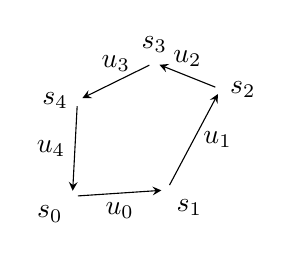
\begin{tikzpicture}[scale=.8,>=stealth]
\coordinate (a) at (0,0); \coordinate (b) at (1.5,.1); \coordinate (c) at (2.35,1.7);
\coordinate (d) at (1.3,2.12); \coordinate (e) at (.08,1.52);
\foreach \p/\q/\lbl/\pos in {a/b/0/below,b/c/1/right,c/d/2/above,d/e/3/above,e/a/4/left}
 {\draw[->,shorten <=2pt,shorten >=2pt] (\p)--(\q) node[midway,\pos] {$u_{\lbl}$};}
\foreach \p/\lbl/\pos in {a/0/below left,b/1/below right,c/2/right,d/3/above,e/4/left}
 {\node[\pos] at (\p) {$s_{\lbl}$};}
\end{tikzpicture}}

% top centre, vertex coordinates and edge coordinates
\[
\begin{aligned}
s_0&=(0,0) & u_0&=(1,0)\\
s_1&=(1,0) & u_1&=(x-1,y)\\
\big[\,\inserted{s_4=(0,f_0)}& & u_2&=(x'-x,y'-y)\\
s_2&=(x,y) & u_3&=(-x',f_0-y')\\
s_3&=(x',y') & u_4&=(0,-f_0)
\end{aligned}
\]

% upper right, seven lines
\[
\begin{aligned}
f_1&=y\\
f_2&=\underbrace{\underbrace{(\deleted{x'}x-\deleted{x}1)(y'}-y)}-y(\underline{x'}-\underline{x})\\
&=(xy'-yx')\deleted{\unsure{+}}-(y'-y)\\
f_3&=\underbrace{(x'-\underbrace{x)(f_0-y')}}+x'(\underline{y'}-\underline{y})\\
&=(xy'-yx')+f_0(x'-x)\\
f_4&=f_0x'\\
f_0&=f_0
\end{aligned}
\]

% upper middle, first brace and adjacent expression
\[
\left\{\begin{aligned}
\deleted{\unsure{y'}}y&=f_1 &&\deleted{y'=}\\
x'&=f_4/f_0\\
xy'-y'&=f_2+f_1f_4/f_0-f_1\\
xy'\deleted{\unsure{+}}-f_0x&=f_3+f_1f_4/f_0-f_4
\end{aligned}\right.
\qquad f_0x-y'=-f_1+f_2-f_3+f_4
\]

% middle, second brace and two definitions to right
{\scriptsize
\[
\left\{\begin{aligned}
y&=f_1\\
x'&=f_4/f_0\\
y'&=f_0x+{\unsure{\gamma|\chi|y|X}}_1^4
\end{aligned}\right.
\quad \gamma_1^4=f_1-f_2+f_3-f_4
\quad \gamma=f_0-f_1+f_2-f_3+f_4=\deleted{\unsure{1}}f_0-\gamma_1^4
\]
}

% middle and lower middle, substitution then quadratic
\[
\begin{aligned}
x(f_0x+\gamma_1^4)-f_0x-\gamma_1^4&=f_2+f_1f_4/f_0-f_1\\
f_0x^2+\underset{-\gamma}{\underline{(\gamma_1^4-f_0)}}x
&-(\deleted{f_1}-\deleted{f_2}+f_3-f_4+\deleted{f_2}+f_1f_4/f_0-\deleted{f_1})\\
\deleted{\unsure{x^2}}\,\cdot\, f_0x^2-\gamma x&+(f_4-f_3-f_1f_4/f_0)
\qquad \gamma=1-\gamma_1^4
\end{aligned}
\]

% lower half, root and unfinished expression
\[
x=\frac{1}{2f_0}\left(\gamma\pm\sqrt{\gamma^2-4(f_0f_4-f_0f_3-f_1f_4)}\deleted{\unsure{/f_0}}\right)
\qquad \gamma=
\]

% lower half, four-line expansion
\[
\begin{aligned}
\gamma^2={}&f_0+f_1^{\unsure{2|1}}+f_2^2+f_3^2+f_4^2-2f_0f_1+2f_0f_2
\deleted{\unsure{+}}-2f_0f_3+2f_0f_4\\
&-2f_1f_2+2f_1f_3-2f_1f_4\\
&\deleted{\unsure{+}}-2f_2f_3+2f_2f_4\\
&-2f_3f_4
\end{aligned}
\]

% bottom third, Δ, boxed pair products
\[
\begin{aligned}
\Delta={}&f_0^2+f_1^2+f_2^2+f_3^2+f_4^2-\underset{\longrightarrow}{\boxed{2f_0f_1}+\boxed{2f_0f_2}}+\boxed{2f_0f_3}-\boxed{2f_0f_4}\\
&-\boxed{2f_1f_2}+\underline{\boxed{2f_1f_3}}+2\underset{\longrightarrow}{\boxed{f_1f_4}}\\
&-\underset{\longleftarrow}{\boxed{2f_2f_3}}+\underline{\boxed{2f_2f_4}}\\
&-\boxed{2f_3f_4}
\end{aligned}
\]

% bottom third, sums at left and beneath
\[
\begin{aligned}
&=\sum f_i^2-2\sum f_i f_{i+1}+2\sum f_{i-1}f_{i+\unsure{1|2}}\\
&=\sum f_{\unsure{i|i0}}^2+2\sum f_{i+1}(f_i-f_{i-1})\\
&(f_0-f_1+f_2+f_3-f_4)^2\\
&\qquad+4(f_1f_3+f_2f_3+f_2f_4)
\end{aligned}
\]

% below bottom dividing line
\noindent\rule{\linewidth}{.3pt}
{\small
\[
u_3\wedge u_4-u_2\wedge u_3=u_3\wedge u_4+u_3\wedge u_2=u_3\wedge(u_2+u_4)
\qquad (u_4\wedge u_0)(u_3\wedge(u_2+u_4))-
\]
}

% archive sheet number: 26
\scanpage{21}
\mspage{8}

% top left, four lines
\[
\begin{aligned}
&x^2+y^2+z^2+2yz+2zx-2xy=\\
&\deleted{{\unsure{\xi|\zeta}}^2+\eta^2+2(\xi+\eta)}+\\
&\xi^2+\eta^2-2\xi\eta+2(\xi+\eta)+1\\
&(\underbrace{\xi-\eta}_{\unsure{u|U}})^2+2(\underbrace{\xi+\eta}_{\unsure{v|V}})+1
\end{aligned}
\]

% upper left, below sloping rule
\figure{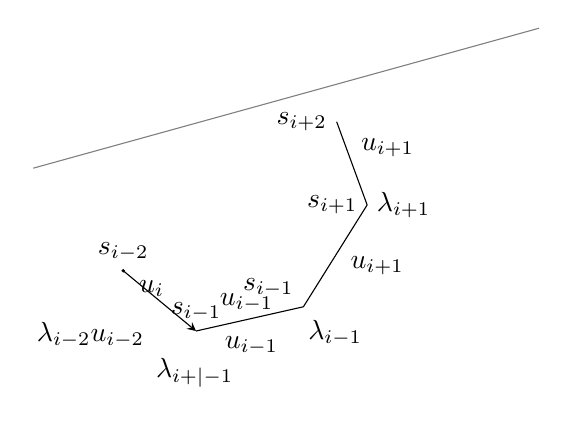
\begin{tikzpicture}[scale=.88,>=stealth]
\draw[gray,thin] (-1.3,2.48)--(6,4.5);
\coordinate (a) at (0,1.0); \coordinate (b) at (1.05,.13); \coordinate (c) at (2.6,.48); \coordinate (d) at (3.52,1.95); \coordinate (e) at (3.08,3.15);
\fill (a) circle (.8pt); \draw[->] (a)--(b); \draw (b)--(c) (c)--(d) (d)--(e);
\node[above] at (a) {$s_{i-2}$}; \node[above] at (b) {$s_{i-1}$};
\node[above left] at (c) {$s_{i\deleted{\unsure{-1}}}$};
\node[left] at (d) {$s_{i+1}$}; \node[left] at (e) {$s_{i+2}$};
\node at (.41,.74) {$\deleted{\unsure{u_{i}}}$};
\node[below left] at (.44,.4) {$\lambda_{i-2}u_{i-2}$};
\node[above] at (1.78,.26) {$\deleted{\unsure{u_{i-1}}}$}; \node[below] at (1.85,.19) {$u_{i-1}$};
\node[below] at (1.03,-.12) {$\lambda_{i\unsure{+|-}1}$};
\node[below right] at (2.53,.43) {$\lambda_{i\deleted{\unsure{-1}}}$};
\node[right] at (3.14,1.07) {$u_{i\deleted{\unsure{+1}}}$}; \node[right] at (d) {$\lambda_{i+1}$};
\node[right] at (3.29,2.77) {$u_{i+1}$};
\end{tikzpicture}}

% above boxed recurrence
\[
\deleted{\lambda_{i+1}u_i-\lambda_{i+2}(u_{i+1}+u_{i+2})+\lambda_{i+3}u_{i+3}}=0
\]

% middle, boxed
\[
\boxed{\lambda_{i-1}u_{i-2}-\lambda_i(u_{i-1}+u_i)+\lambda_{i+1}u_{i+1}=0}
\]

% middle left
\figure{\begin{tikzpicture}[scale=.83,>=stealth]
\draw[->] (0,0)--(1.45,-.04) node[midway,below] {$u_0$};
\node[below left] at (0,0) {$s_0$}; \draw[->] (1.56,.03)--(2.18,1.33) node[midway,right] {$u_1$};
\draw[->] (2.14,1.49)--(1.77,2.60) node[midway,right] {$u_2$};
\node at (.16,2.25) {$\deleted{\unsure{x}}$};
\end{tikzpicture}}

% middle right
\[
\underbrace{u_0\quad u_1}_{\text{base}}\qquad u_2=\unsure{\xi|x}u_0+\unsure{y|\eta}u_1
\]

% middle right, expressions for u₃,u₄,u₅
\[
\begin{aligned}
u_3&=\frac1{\lambda_3}\big(\lambda_2(u_1+u_2)-\lambda_1u_0\big)\\
u_4&=\frac1{\lambda_3\lambda_4}\big(\hspace{4em}-\\
u_5&=\frac1{\lambda_3\lambda_4\lambda_5}\big(\quad\rule{5em}{.35pt}\quad\big)
\end{aligned}
\]

% lower left beside u₅
\figure{\begin{tikzpicture}[scale=.75,>=stealth]
\draw[->] (0,.75)--(.86,.06); \draw[->] (.92,0)--(1.72,0); \draw (1.72,0)--(1.96,0); \fill (1.96,0) circle (2pt);
\draw[->] (2.08,0)--(3.05,0); \draw[->] (3.12,.12)--(3.68,1.12);
\end{tikzpicture}}

% lower left, above last polygon
\figure{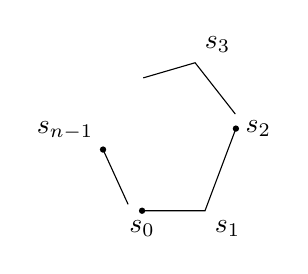
\begin{tikzpicture}[scale=.74]
\draw (0,1.05)--(.43,.11) (.67,0)--(1.75,0)--(2.28,1.41)
 (2.27,1.66)--(1.58,2.54)--(.69,2.28);
\foreach \p in {(0,1.05),(.67,0),(2.28,1.41)}{\fill \p circle (1.55pt);}
\node[above left] at (0,1.05) {$s_{n-1}$}; \node[below] at (.67,0) {$s_0$};
\node[below right] at (1.75,0) {$s_1$}; \node[right] at (2.28,1.41) {$s_2$}; \node[above right] at (1.58,2.54) {$s_3$};
\end{tikzpicture}}

% lower right, two lines
\[
\begin{aligned}
u_{n-1}&=\frac{\lambda_{n-2}}{\lambda_3\,\text{--}\,\lambda_{n-1}}
 \left(P_{n-1}u_0+\unsure{Q|B}_{n-1}u_1+R_{n-1}u_2\right)\\
u_i&=\frac{1}{\lambda_3\lambda_{\unsure{4|5}}\lambda_i}
 P_i(\lambda_1-\lambda_{i-1})u_0+\unsure{Q_i|b_i}\,\lambda_1-
\end{aligned}
\]

% foot left
\figure{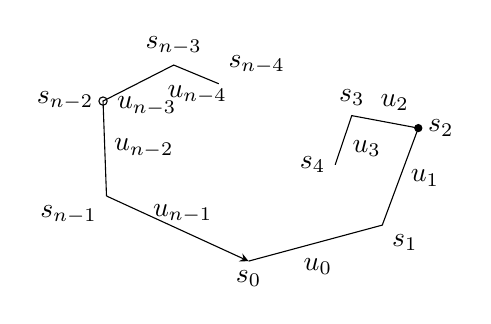
\begin{tikzpicture}[scale=.88,>=stealth]
\coordinate (a) at (2.27,0); \coordinate (b) at (4.20,.52); \coordinate (c) at (4.72,1.92);
\coordinate (d) at (3.76,2.10); \coordinate (e) at (3.52,1.39); \coordinate (f) at (1.84,2.56);
\coordinate (g) at (1.19,2.83); \coordinate (h) at (.17,2.31); \coordinate (j) at (.22,.94);
\draw (a)--(b)--(c)--(d)--(e) (f)--(g)--(h)--(j); \draw[->] (j)--(a);
\fill (c) circle (1.7pt); \draw (h) circle (1.7pt);
\foreach \p/\lbl/\pos in {a/0/below,b/1/below right,c/2/right,d/3/above,e/4/left,f/{n-4}/above right,g/{n-3}/above,h/{n-2}/left,j/{n-1}/below left}
 {\node[\pos] at (\p) {$s_{\lbl}$};}
\node[below] at (3.27,.18) {$u_0$}; \node[right] at (4.47,1.20) {$u_1$}; \node[above] at (4.38,2.03) {$u_2$};
\node[right] at (3.63,1.63) {$u_3$}; \node[below] at (1.53,2.67) {$u_{n-4}$};
\node[below] at (.80,2.51) {$u_{n-3}$}; \node[right] at (.19,1.63) {$u_{n-2}$}; \node[above] at (1.32,.41) {$u_{n-1}$};
\end{tikzpicture}}

% archive sheet number: 27
\scanpage{22}
\mspage{9}

\begingroup
\makeatletter
\tagsleft@true
\makeatother

% top, short first line and long second line
{\scriptsize
\[
\begin{aligned}
u_3&=1/\lambda_3\,(P_3u_0+Q_3u_1+R_3u_{\unsure{3|2}})\\
u_i&=\frac{\lambda_{i-1}}{\lambda_3\lambda_4\cdots\lambda_i}
 \big(P_i(\lambda_1,\text{--},\lambda_{i-1})u_0+
 Q_i(\lambda_1,\text{--},\lambda_{i-1})u_1+
 R_i(\lambda_1,\text{--},\lambda_{i-1})u_2\big)\\
&\hspace{10em}(i\geq4)
\end{aligned}
\]
}

% upper quarter, three-line substitution
{\scriptsize
\[
\begin{aligned}
\lambda_{i+1}u_{i+1}
 &=\lambda_i(u_i+u_{i\unsure{+|-}1})-\lambda_{i-1}u_{i-2}\\
 &=\frac{1}{\lambda_3\text{--}\lambda_{i-2}}[P_i u_0+Q_i u_1+R_i u_2]
 +\frac{\lambda_i\lambda_{i-2}}{\lambda_3\text{--}\lambda_{i-1}}[P_{i-1}u_0+Q_{i-1}u_1+R_{i-1}u_2]\\
 &\quad-\frac{\lambda_{i-1}\lambda_{i-3}}{\lambda_3\lambda_4\text{--}\lambda_{i-2}}[P_{i-2}u_0+Q_{i-2}u_1+R_{i-2}u_2]
\end{aligned}
\]
}

% upper middle, empty indexed square brackets
\[
u_{i+1}=\frac{\lambda_i}{\lambda_3\text{--}\lambda_{i+1}}
\left\{\lambda_{i-1}[\,]_1+\lambda_i\lambda_{i-2}[\,]_2
\deleted{\unsure{+}}-\lambda_{i-1}^2\lambda_{i-3}\unsure{\lambda}[\,]_3\right\}
\]

% above recurrence box
\diagram{$\begin{array}{ccccc}
i-3,&i\deleted{\unsure{+}}-2,&i-1,&i,&i+1\\
0&-1&\underline{1}&0&-1
\end{array}$}

% centre, framed recurrence and condition
\[
\boxed{\begin{gathered}
\left\{\begin{aligned}
P_{i+1}&=\lambda_{i-1}P_i+\lambda_i\lambda_{i-2}\deleted{\unsure{R}}P_{i-1}-\lambda_{i-1}^2\lambda_{i-3}\deleted{\unsure{R}}P_{i-2}\\
Q_{i+1}&=\lambda_{i-1}Q_{\unsure{i|j}}+\lambda_i\lambda_{i-2}Q_{i-1}-\lambda_{i-1}^2\lambda_{i-3}\deleted{\unsure{R}}Q_{\unsure{i|0}-2}\\
R_{i+1}&=\lambda_{i-1}R_i+\lambda_i\lambda_{i-2}R_{i-1}-\lambda_{i-1}^2\lambda_{\unsure{i|1}-3}R_{i-2}
\end{aligned}\right.\\
\deleted{\unsure{5\leq i}}\qquad i\geq6
\end{gathered}}
\]

% centre below box, initial forms
\[
\begin{aligned}P_3&=-\lambda_1\\Q_3&=\lambda_2\\R_3&=\lambda_2\end{aligned}
\qquad\Big/\quad
\begin{gathered}P_i,Q_i,R_i\ \text{\uline{formes}}\\
\text{de degré }i-3\quad(i\geq4)\end{gathered}
\]

% lower half, sum of the uᵢ, struck coefficient expressions
{\scriptsize
\[
\begin{aligned}
(\lambda_3\text{--}\lambda_{n-1})\sum_0^{n-1}u_i
&=\deleted{\underbrace{\left(\sum_{i=0}^{n-1}P_i(\lambda_1\text{--}\lambda_{n-2})\right)}u_0+(\qquad)u_1+(\qquad)u_2}\\
&\quad\widetilde P_{n-1}(\lambda_1\text{--}\lambda_{n-2})u_0+
 \widetilde Q_{n-1}(\lambda_1\text{--}\lambda_{n-2})u_1+
 \widetilde R_{n-1}(\lambda_1\text{--}\lambda_{n-1})u_2
\end{aligned}
\]
}

% lower third, long struck line
\[
\deleted{\widetilde P_{n-1}(\lambda_1\text{--}\lambda_{n-2})u_0+
\widetilde Q_{n-1}(\quad)u_1+\widetilde R_{n-1}(\quad)u_2=0}
\]

% lower third, expansion of tilde P
\[
\begin{aligned}
\widetilde P_{n-1}(\lambda_1,\text{--}\lambda_{n-2}) &=
(\lambda_3\text{--}\lambda_{n-1})+
\deleted{\sum_{i=3}^{\unsure{n-1}}\lambda_{i-1}\lambda_{\unsure{i+1|j+1}}\lambda_{i}\text{--}}\\
&\quad\big(\lambda_4\lambda_5\text{--}\lambda_{n-1}P_3
 +\lambda_3\lambda_5\lambda_6\text{--}\lambda_{n-1}P_4\\
&\qquad+\lambda_{4}\lambda_6\lambda_7\text{--}\lambda_{n-1}P_5\unsure{\longleftarrow|+\text{---}}\big)
\end{aligned}
\]

% before ring assertion
\unsure{etc}

% near foot
\[
\widetilde P_{n-1}\in\mathbb Z[\Lambda_1,\text{--}\Lambda_{n-1}]
\]

% bottom box, label on left (0)
\[
\deleted{\unsure{\sum}}\quad
\boxed{\widetilde P_{n-1}u_0+\widetilde Q_{n-1}u_1+\widetilde R_{n-1}u_2=0}\tag*{(0)}
\]

\endgroup

% archive sheet number: 28
\scanpage{23}
\mspage{10}

\begingroup
\makeatletter
\tagsleft@true
\makeatother

% top line
\[
\deleted{u_n=\lambda P_n(\lambda_1,\text{--},\underset{\substack{\Vert\\\lambda_0}}{\lambda_n})u_0+}
\]

% upper part, full uₙ formula
{\scriptsize
\[
\begin{aligned}
\underset{\substack{\Vert\\u_0}}{u_n}
&=\frac{\lambda_{n-1}}{\lambda_3\text{--}\lambda_{n-1}\underset{\substack{\Vert\\\lambda_0}}{\underline{\lambda_n}}}
\Big[P_n(\lambda_1,\text{--},\unsure{\lambda_{n-1}|n-1},\underset{\substack{\Vert\\\lambda_{\unsure{0|3}}}}{\lambda_n})u_0+
Q_n(\lambda_1,\text{--},\underset{\substack{\Vert\\\lambda_0}}{\lambda_n})u_1+
R_n(\lambda_1\text{--}\underset{\substack{\Vert\\\lambda_0}}{\lambda_n})u_2\Big]\\
&=u_0\qquad \text{i.e.}
\end{aligned}
\]
}

% first frame, label at left
{\scriptsize
\[
\boxed{\big[\lambda_{n-1}P_n-(\lambda_3\text{--}\lambda_{n-1}
\underset{\substack{\Vert\\\lambda_0}}{\underline{\lambda_n}})\big]u_0+
\lambda_{n-1}Q_n(\quad)u_1+\lambda_{n-1}R_n(\quad)u_2=0}\tag*{(1)}
\]
}

% below first frame
\[
\begin{aligned}
\underset{\substack{\Vert\\u_1}}{u_{n+1}}&=\frac{\lambda_n}{\lambda_3\text{--}\lambda_{n+1}}
\Big[P_{n+1}(\lambda_1,\text{--},\lambda_{n-1},\underset{\substack{\Vert\\\lambda_0}}{\lambda_n},
\underset{\substack{\Vert\\\lambda_1}}{\lambda_{n+1}})u_0\ \unsure{+\text{---}|\text{---}}\Big]\\
&=u_1.\qquad\text{\unsure{i.e.|''---.}}
\end{aligned}
\]

% second frame, label at left
{\scriptsize
\[
\boxed{\lambda_nP_{n+1}(\quad)u_0+
\big(\lambda_n Q_{n+1}-(\lambda_3\lambda_4\cdots\lambda_{n+1})\big]u_1+
\lambda_n R_{n+1}(\quad)\underset{\substack{\Vert\\0}}{u_2}}\tag*{(2)}
\]
}

% between second and third frame
\[
u_{n+2}=\frac{\lambda_{n+1}}{\lambda_3\text{--}\lambda_{n+2}}
 [P_{n+1}u_0+Q_{n+2}u_1+R_{n+2}u_2]=u_2
\]

% third frame, label at left
{\scriptsize
\[
\boxed{\begin{aligned}
\lambda_{n+1}P_{n+2}(\quad)u_0+\lambda_{n+1}Q_{n+2}(\quad)u_1+
\lambda_{n+1}R_{n+2}(-)(\lambda_3\text{--}\lambda_{n+2})u_2\\
=0
\end{aligned}}\tag*{(3)}
\]
}

% left of last frame
i e

% upper border of bottom frame
\[
\deleted{A\,\unsure{A}\qquad A_0(\lambda_1\text{--}\lambda_{n-2})u_0+A_1(}
\]

% bottom frame, four lines
{\scriptsize
\[
\boxed{\begin{aligned}
A_0^{\unsure{n|u}}(\lambda_1,\text{--}\lambda_{n-2})u_0+
\deleted{A}B_0^n(\lambda_1\text{--}\lambda_{n-2})u_1+C_0^n(\lambda_1\text{--}\lambda_{n-2})u_2&=0\\
A_1^n(\lambda_0,\text{--},\lambda_{n-1})u_0+
\deleted{A}B_1^n(\lambda_0,\text{--}\lambda_{n-1})u_1+
C_1^n(\lambda_0,\text{--}\lambda_{n-1})u_2&=0\\
A_2^n(\qquad)u_0+\deleted{\unsure{R|A}}B_2^n(\deleted{\unsure{\lambda}}\text{---})u_1+C_2^n(\qquad)u_2&=0\\
A_3^n(\qquad)u_0+B_3^n(\qquad)u_1+C_3^n(\qquad)u_{\unsure{2|0}}&=0
\end{aligned}}\tag*{(\unsure{E|e|*})}
\]
}

\endgroup

% archive sheet number: 29
\scanpage{24}
\mspage{11}

% top, rings one above the other
\[
\begin{aligned}
A_i^{\unsure{n|u}},B_i^n,C_i^n&\in\mathbb Z[\Lambda_0,\text{--},\Lambda_{n-1}]\\
&\hspace{3.2em}\cup\\
A_0^n,B_0^n,C_0^n&\in\mathbb Z[\Lambda_1,\text{--},\Lambda_{n-2}]
\end{aligned}
\]

% above NB, crossed line
\deleted{\unsure{Quand|Prenons} $\lambda_3=1$, \unsure{les autres} $\lambda_i$ $(i\geq4$}

% upper third, NB, uniqueness paragraph
\uline{NB} \unsure{Et.|Étt|Si} \inserted{\unsure{le polygone fixé, les} $u_i$ \unsure{(}$0\leq i\leq n-1$) \uline{et}} $\lambda_1\ \lambda_2\ \lambda_3$ fixés, \deleted{\unsure{ainsi que}} si de plus on suppose tous les \inserted{$u_i$ et les} $\lambda_i$ $(0\leq i\leq n-1)\ne0$, alors les $\lambda_i$ $(4\leq i\leq n-1)$ sont déterminés de façon unique. D'ailleurs la relation

% just above drawing
\[
\lambda_1u_0-\lambda_2(u_1+u_2)+\lambda_3u_3=0
\]

% middle right, beside drawing
montre que, si $u_0,\ u_1+u_2=u_1^3,\ u_3$ ne sont pas coll., alors les $(\lambda_1;\lambda_2,\lambda_3)$ possibles (pour cette relation) \unsure{font|forment} un espace de dim $1$, \unsure{resp.|i.e.} \deleted{\unsure{0}}.

% middle left
\figure{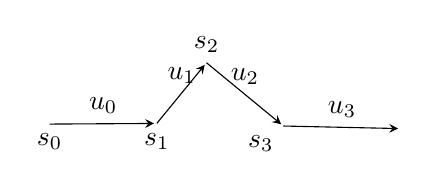
\begin{tikzpicture}[scale=.82,>=stealth]
\coordinate (a) at (0,0); \coordinate (b) at (1.66,.01); \coordinate (c) at (2.43,.95); \coordinate (d) at (3.62,-.03); \coordinate (e) at (5.44,-.07);
\foreach \p/\q/\i in {a/b/0,b/c/1,c/d/2,d/e/3}{\draw[->,shorten >=1pt] (\p)--(\q) node[midway,above] {$u_{\i}$};}
\node[below] at (a) {$s_0$}; \node[below] at (b) {$s_1$}; \node[above] at (c) {$s_2$}; \node[below left] at (d) {$s_3$};
\end{tikzpicture}}

% middle to lower part
$(\lambda_1,\lambda_2,\lambda_3)$ est \unsure{déterminé} mod \unsure{homothétie} par polygone -- donc aussi $(\lambda_0,\text{--}\lambda_{n-1})$. Changeant les rôles par \unsure{renumérotation|commutation|permutation}, on voit qu'il en est ainsi dès qu'il existe $i$, avec $u_i,\ u_{i+1}+u_{i+2},\ u_{i+3}$ non collin. Mais quand peut-on avoir \deleted{\unsure{les}} \unsure{vect.} coll $\forall i$ !

% lower right above coefficient calculations
\margin{OBS $u_0,u_1$ lin. indép.}

% foot, first pair of systems
\[
\begin{aligned}u_1+u_2&=-\alpha u_0\\u_3&=\beta u_0\end{aligned}
\qquad\left\{\begin{aligned}u_2&=-\alpha u_0-u_1\\u_3&=\beta u_0\end{aligned}\right.
\]

% foot, second pair and conclusions at right
\[
\begin{aligned}\deleted{\unsure{u_1|\alpha}}u_2+u_3&=\gamma u_1\\u_4&=\delta u_1\end{aligned}
\quad\text{i.e}\quad
\left\{\begin{aligned}u_3&=\alpha u_0+(1+\gamma)u_1\\u_4&=\delta u_1\end{aligned}\right.
\qquad\begin{aligned}\gamma&=-1\\\beta&=\alpha\end{aligned}
\]

% archive sheet number: 30
\scanpage{25}
\mspage{12}

% top left
\[
\begin{aligned}
u_2&=-\alpha u_0-u_1\\u_3&=\unsure{-}\alpha u_0\\u_4&=\delta u_1
\end{aligned}
\]

% upper centre
\[
u_{i+3}=\alpha_i u_i
\]

% left beside slashed u₀ and u₁
\figure{\begin{tikzpicture}[scale=.83,>=stealth]
\draw[->] (0,0)--(1.38,-.57); \draw (1.48,-.58)--(3.22,-.16) (3.29,-.2)--(5.22,-1.04);
\end{tikzpicture}}

% upper middle, slashes and eight vector rows
\[
\begin{aligned}
&u_0\ \big/\ u_1\ \big/\\
u_2&=-\alpha_0u_0-u_1\\
u_3&=\alpha_0u_0\\
u_4&=\alpha_1u_1\\
u_5&=\alpha_2(\unsure{-}\alpha_0u_0-u_1)\\
u_6&=\alpha_3\alpha_0u_0\\
u_7&=\alpha_4\alpha_2(-\alpha_0u_0-u_1)\\
u_8&=\alpha_5\alpha_3\alpha_0u_0\\
u_9&=\alpha_6\alpha_4\alpha_2(-\alpha_0u_0-u_1)
\end{aligned}
\]

% left of u₇ row
\margin{$=$}

% just below fold, left and right
\[
\left.\begin{aligned}u_0\\u_1\end{aligned}\right\}\ \text{lin. indép}
\quad\Big|\quad
\begin{aligned}
&\Rightarrow (u_1,u_2)\ \text{lin. indép}\\
&\quad\text{\unsure{donc} (\unsure{tous les|$\forall i$|tous} $(\unsure{u_i,u_{i+1}})$ lin. indép)}
\end{aligned}
\]

% lower half, two columns
\[
\begin{aligned}
u_2&=-\deleted{\alpha}\beta_0u_0-u_1 &(\ \beta_0&=\alpha_0\qquad\unsure{\text{si}|b_i|\text{et}}\\
u_3&=\deleted{\alpha}\beta_0u_0\\
u_4&=\beta_1u_1 &\beta_{1}&=\alpha_1\\
u_5&=\beta_2u_2 &\beta_2&=\alpha_2\\
u_6&=\beta_3u_0 &\beta_3&=\alpha_3\alpha_0\\
u_7&=\beta_4u_2
\end{aligned}
\]

% below list, irregular enclosure
\[
\boxed{\begin{aligned}
&&\underline{u_0},\,\underline{u_2}\quad &\text{lin. indép}\\
u_1&=-u_2-\beta_0u_0\\
u_3&=\beta
\end{aligned}}
\]

% bottom quarter, right
\[
\begin{aligned}
u_3+u_4&=\beta_0u_0+\beta_1u_1\quad //\, u_2=-\beta_0u_0\deleted{\unsure{+}}-u_1\\
&&\beta_1=1
\end{aligned}
\]

% bottom, interrupted reasoning
\deleted{donc}
\[
u_{\unsure{i|2}}=u_{i+3}\qquad\deleted{u_0\,u_1\,u_2}\qquad\text{i.e}\quad u_1=u_4
\]

% last line before repeating row
donc $n\equiv0\ (3)$ (\unsure{sinon} $u_i=u_{i+1}=\text{--}\quad\forall i$ exclu \unsure{---})

% foot, running into lower edge
\[
\underset{\unsure{1}}{u_0}\quad u_1\quad u_2\quad
\underset{\substack{\Vert\\u_3}}{u_0}\quad\underset{\substack{\Vert\\u_4}}{u_1}\quad
\underset{\substack{\Vert\\u_5}}{u_2}\quad\underset{\substack{\Vert\\u_6}}{u_0}\quad
\underset{\substack{\Vert\\u_7}}{u_1}\quad\underset{\substack{\Vert\\u_8}}{u_2}\quad\text{---}
\]

% archive sheet number: 31
\scanpage{26}
\mspage{13}

\begingroup
\makeatletter
\tagsleft@true
\makeatother

% top, parallelism and computation
\[
\begin{aligned}
u_1+u_2&\ //\ u_0 &u_2&=\alpha_0u_0-u_1\\
u_2+u_0&\ //\ u_1 &u_2+u_0&=(1+\alpha_0)u_0-u_1\qquad //\ u_1\\
u_0+u_1&\ //\ u_2 &&\text{i.e.}\quad1+\alpha_{\unsure{0|\alpha}}=0\qquad\alpha_0=-1\\
&&u_2&=-u_0-u_1
\end{aligned}
\]

% upper middle, underlined heading and statement
\uline{Proposition} Soit $u_*=(u_i)_{i\in\mathbb Z/\deleted{\unsure{\mathbb Z}}n\mathbb Z}$ un syst. de $n$ vecteurs \inserted{tous} \uline{non nuls} du plan vectoriel $V$, \deleted{\unsure{munis}} \deleted{\uline{\unsure{formant base|de somme nulle}}}, et \deleted{supposons qu'il existe} \inserted{considérons l'ens \inserted{$N(u_*)$} des} $(\lambda_i)_{i\in\mathbb Z/n\mathbb Z}$ dans $k^{\mathbb Z/n\mathbb Z}$ tels que l'on \deleted{\unsure{soit}} ait les relations

% below statement, cyclic constraint
\[
\lambda_i u_{i-1}-\lambda_{i+1}(u_i+u_{i\unsure{-|+}1})+\,\unsure{\cdot}\,\lambda_{i+2}u_{i+2}=0
\qquad\forall i\in\mathbb Z/n\mathbb Z \tag*{($\unsure{\alpha|*}$)}
\]

% middle, before list
\deleted{\unsure{$1^{\rm o}$} Alors $N$ \unsure{est un} sous-espace vectoriel de \unsure{$k^n$}} \inserted{Conditions équivalentes} \inserted{(\unsure{$k$ le corps|le noyau})}

% condition a, upper lines
\deleted{\uline{Supposons} que} \textcircled{a}\quad $\exists\,(\lambda_i)\in N(u_*)$ tel que \uline{tous} les $\lambda_i$ \deleted{sont} $\ne0$, \deleted{\unsure{et dim} $N(u_*)\geq1)$} \deleted{\unsure{Pour que}} \uuline{et}

% condition a, heavily crossed block
\deleted{$\dim N(u_*)\geq2$, il \unsure{f.} et \unsure{s.} que \unsure{l'on ait les} conditions suivantes a) $u$}

% condition a, right of cancellation
\[
\dim_k N(u_*)\geq2
\]

% condition b
\textcircled{b}\quad $\forall i,\quad u_i,\ u_{i+\unsure{1|0}}+u_{i+\unsure{3|2}}\quad u_{i+3}$ sont col.

% condition c
\[
\text{\textcircled{c}}\quad\forall i,\quad\text{--}\quad
\left\{\begin{aligned}
u_{i+3}&=u_i\ \deleted{\unsure{\text{pour tout }i}}\ \deleted{u_0+u_1+u_2=0}\\
u_{i+1}+u_{i+2}&=-u_i.\qquad \forall i
\end{aligned}\right.
\]

% condition d
\[
\text{\textcircled{d}}\quad
\left\{\begin{aligned}
\forall i,\ \text{--}\quad &u_i=u_{i+3}\qquad\deleted{\unsure{(\Rightarrow n\equiv0\ (3))}}\\
&u_0+u_1+u_2=0
\end{aligned}\right.
\]

\endgroup

% archive sheet number: 32
\scanpage{27}
\mspage{14}

% top centre, above proof
\margin{\unsure{OPS|OBS} $k$ infini}

% upper third
\uline{Dém} Un $(\lambda_i)\in N(u_*)$ tel que les comp. sont $\ne0$ est connu \unsure{quand} on \unsure{connait|connaît} trois comp. consécutives, disons $\lambda_1,\lambda_2,\lambda_3$ (on utilise le fait que les $u_i$ sont $\ne0$), \deleted{et on en conclut} i.e.

% upper middle, two-line map
\diagram{\begin{tikzcd}[ampersand replacement=\&,row sep=2pt,column sep=large]
N(u_*)\arrow[r,dash] \& k^3\\
(\lambda_i)\arrow[r,mapsto] \&(\lambda_1,\lambda_2,\lambda_3)
\end{tikzcd}}

% right of map
a un noyau

% left margin rising to the right
% slanted
\margin{Lemme (si $N(u_*)\not\subset\bigcup H_i$)}

% middle, heavily reworked sentence
\uline{\unsure{V|v}}\quad \inserted{\unsure{dont de quelque translaté|dont des translatés} \deleted{de} $N(u_*)$} \unsure{contenu|contenus} \deleted{dans} la réunion des hyperplans $H_i$ \deleted{d'équations} \inserted{\unsure{séparés|sép.} par un pt} \unsure{de coordonnées|d'ordonnées|d'équations} $\lambda_i=0$ $(i\in\mathbb Z/n\mathbb Z)$ -- donc, $k$ étant infini, \deleted{\unsure{l'on a bien}} ce noyau est réduit à un pt, i.e. est nul. Donc

% centre, injectivity and bounds
$N(u_*)\to k^3$ est \uline{injectif}. Donc $1\leq\dim N(u_*)\leq3$. Mais \deleted{\unsure{OPS} \unsure{quelques} $u_i$}

% lower half
On a $\dim N(u_*)\ne3$, i.e. $N(u_*)\mathbin{\unsure{-|\to}}k^3$ n'est pas surjectif -- \deleted{il} \inserted{l'image} ne contient pas p.ex $(1,0,0)$ (car $\lambda_1u_0\deleted{\unsure{+}}-\lambda_2(u_1+u_2)+\lambda_3u_3$ implique $u_0=0$, \unsure{contraire|contrmt} à l'hyp. On veut regarder le cas $\dim N(u_*)=2$. On

% lower third, image and kernel
{\small
\[
\begin{aligned}
\deleted{N(u_*)\longrightarrow}\quad N(u_*)&\simeq\operatorname{Im}(N(u_*)\to k^3)
 \subset\{(\lambda_1,\lambda_2,\lambda_3)\mid\lambda_1u_0-\lambda_2(u_1+u_2)\\
&\hspace{23em}+\lambda_3u_3=0\}\\
\deleted{\text{donc}}\quad &=\operatorname{Ker}\big((\lambda_1,\lambda_2,\lambda_2)\mathbin{\unsure{-|\to|\mapsto}}\lambda_1u_0-\lambda_2(u_1+u_2)+\lambda_3u_3\big)
\end{aligned}
\]
}

% bottom, dimensions and two cases
\[
\begin{aligned}
\text{donc}\quad\dim N(u_*)&\leq\dim\operatorname{Ker}=\deleted{\unsure{f}}3-
\deleted{\unsure{\dim}}\operatorname{rg}(u_0,u_1+u_2,u_3)\\
&=\begin{cases}1&\text{si }\mathrm{rg}=2\\2&\text{si }\mathrm{rg}=1\end{cases}
\end{aligned}
\]

% archive sheet number: 33
\scanpage{28}
\mspage{15}

% top two lines
\[
\begin{aligned}
\text{donc}\quad\mathrm{rg}\,N(u_*)=2&\Rightarrow
 \mathrm{rg}(u_i,u_{i+1}+u_{i+2},u_{i+3})=1\\
&&\forall i
\end{aligned}
\]

% below top implication
Donc $a)\Rightarrow b)$. Un calcul \unsure{fait|facile} plus haut montre

% below Un calcul
\[
b)\Longleftrightarrow c)
\]

% next two lines
et on voit \unsure{tout} de suite que \unsure{c'est|c)|ceci} \unsure{équivt|équivaut} à $d)$.

% centre
\unsure{Or|On} considérons les $(\lambda_i)$ \uline{périodiques} de période $3$, tels que

% above main relation
\[
\deleted{\lambda_0u_0+\lambda_1u_1+\lambda_2}
\]

% centre, relation and lower annotations
\[
\lambda_i u_{i-1}\deleted{\unsure{+}}-\lambda_{i+1}
(\underbrace{u_i+u_{i+1}}_{-u_{i-1}})+
\underset{\substack{\Vert\\\lambda_{i-1}}}{\lambda_{i+2}}
(\underset{\substack{\Vert\\u_{i-1}}}{u_{i+2}})=0\qquad\forall i
\]

% centre, reduction
\[
\text{i.e.}\quad
(\lambda_i+\lambda_{i-1}\deleted{\unsure{u_{i-1}|\lambda_{i-1}}}+\lambda_{i+1})u_{i-1}=0
\]

% final two lines
Ils \unsure{font|forment} un \unsure{vectoriel} de dim $2$ ! Donc $d)\Rightarrow a)$

% archive sheet number: 34
\scanpage{29}
% archive sheet number: 35

\mspage{16}

% top centre
$V$ plan \unsure{vect|vect.} $/k$, $n$ entier $\geq\deleted{\unsure{3|2}}1$

% top, below first line
\uline{Théorème} $u_*=(u_i)_{i\in\mathbb Z/n\mathbb Z}\in{\unsure{V|k}}^{\mathbb Z/n\mathbb Z}$, les $u_i\ne0$

% upper quarter
\[
 N(u_*)=\bigl\{(\lambda_i)\in k^{\mathbb Z/n\mathbb Z}\mid
 \deleted{\sum}\lambda_{\unsure{i|i-1}}u_{i-1}\unsure{-|+}\lambda_i(u_i+u_{i+1})+
 \lambda_{i+1}u_{i-2}=0\qquad\forall i\in\mathbb Z/n\mathbb Z\bigr\}
\]

% below definition
Soit $H_i\subset k^{\mathbb Z/n\mathbb Z}$ hyperplan coord. $i$ ème. On est alors dans les cas \unsure{mutuelt|mutuelmt} exclusifs

% left opposite a
% slanted
\margin{``\uline{Cas général}''}

% upper middle, case a circled
\textcircled{a} $\dim N(u_*)=0$ i.e. $N(u_*)=0$ [i.e., si $\sum u_i=0$, l'application \inserted{can} $\varphi:\unsure{X|\mathcal X}(W)\longrightarrow(\det V)^{\mathbb Z/n\mathbb Z}$ est \uline{lisse} en $u_*$]

% middle, case b circled
\textcircled{b} \deleted{$\dim N(u_*)=1$, \unsure{et|si} \inserted{dim} $N(u_*)=1$ et}

% middle, below cancelled line
\[
 N(u_*)\not\subset\bigcup H_i\quad(\Longrightarrow\ \dim N(u_*)\in\{1,2\})
\]

% left opposite b1
% slanted
\margin{``Cas spécial I''}

% middle, first subcase circled
\[
 \text{\textcircled{$b_1$}}\qquad \dim N(u_*)=1
\]

% left opposite b2
% slanted
\margin{``\uline{Cas hyperspécial}''}

% middle, second subcase circled
\[
 \text{\textcircled{$b_2$}}\qquad \dim N(u_*)=2\quad\Longleftrightarrow
 \left\{\begin{aligned}u_i&=u_{i+3}\\u_0+u_1+u_2&=0\end{aligned}\right.
\]

% left opposite c
% slanted
\margin{``Cas spécial II''}

% below middle, case c and linked outlines
\figure{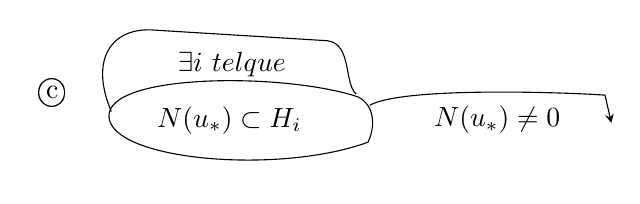
\begin{tikzpicture}[x=1cm,y=.72cm,>=stealth]
\node at (-2.25,-.16) {\textcircled{c}};
\node at (.03,.4) {$\exists i\ \text{tel que}$};
\node at (0,-.58) {$N(u_*)\subset H_i$};
\node at (3.4,-.57) {$N(u_*)\ne0$};
\draw (-1.5,-.42) .. controls (-1.78,.50) and (-1.50,1.05) .. (-.99,1.02)
 -- (1.24,.83) .. controls (1.56,.78) and (1.45,.08) .. (1.61,-.11);
\draw (1.63,-.16) .. controls (.7,.27) and (-1.56,.26) .. (-1.53,-.51)
 .. controls (-1.50,-1.28) and (.62,-1.54) .. (1.76,-.96)
 .. controls (1.86,-.67) and (1.84,-.30) .. (1.63,-.16);
\draw[->] (1.78,-.31) .. controls (2.20,.02) and (4.25,-.08) .. (4.77,-.13)
 -- (4.85,-.62);
\end{tikzpicture}}

% lower third, consequence of c
($\Rightarrow\dim N(u_*)=1$, si $\underset{\ne0}{\lambda}=(\lambda_i)\in N(u_*)$, \deleted{\unsure{donc|avec}} (\unsure{disons}) $\lambda_{i_0}=0$, les \deleted{$\unsure{\lambda|i}$} $i$ tels que $\lambda_i=0$ sont ceux pour lesquels $s_i=s_{i_0}$ (i.e. $u_{i_0}\mathbin{\text{---}}+u_{i-1}=0$)

% lower left, diagonal, three numbered conditions
% slanted
\margin{$\exists O\in E$, droite $\Delta\in E$ \unsure{passant par} $O$, tels que $\forall i$ tels que \unsure{1°)} \deleted{$\lambda_i\ne0$} $u_{i-1}$ \deleted{$\unsure{u_i=0|u_{0i}=0}$} $//\Delta$ et \deleted{$\unsure{u_{i-1}|u_i}$} $u_i\unsure{\longrightarrow|-}//u_{0\unsure{i|2}}$, on \unsure{aura|avant} 2°) $\exists i$, \unsure{un} $s_i\ne0$ 3°) \unsure{du moins} \illegible{2} \unsure{les} $(s_i)$. $\Longleftrightarrow$}

% foot, condition and normalization
Pour qu'on soit dans le cas c, \inserted{où $\lambda_0=0$,} il f et s \deleted{\unsure{que}} que

% foot, conditions a and b
\[
 \begin{aligned}
 &\mathrm a)\quad \sum u_i=0\\
 &\mathrm b)\quad \forall\deleted{\unsure{i|0}}\,1\leq i\leq n-1,\ \text{on ait}\\
 &\hspace{6em} u_{i-1}\,u_i\ //\ u_1\,u_{0i}
 \end{aligned}
\]

% bottom line
et si \inserted{on normalise} $\lambda_1=1$, on aura $\lambda_i$ défini par $u_1u_{0i}=\lambda_i u_i u_{i-1}$\unsure{.}
